\chapter{ANALYTIC NON-EUCLIDEAN GEOMETRY}

We shall use the ordinary polar coördinates, $\rho$ and $\theta$,
and for the rectangular coordinates, $x$ and $y$, of a point, we
shall use the intercepts on the axes made by perpendiculars through
the point to the axes. The formulæ depend upon the trigonometrical
relations, and in our two Geometries differ only in the use of the
imaginary factor $i$ with lengths of lines.

\section{Hyperbolic Analytic Geometry}

\begin{figure}[h]
\centering
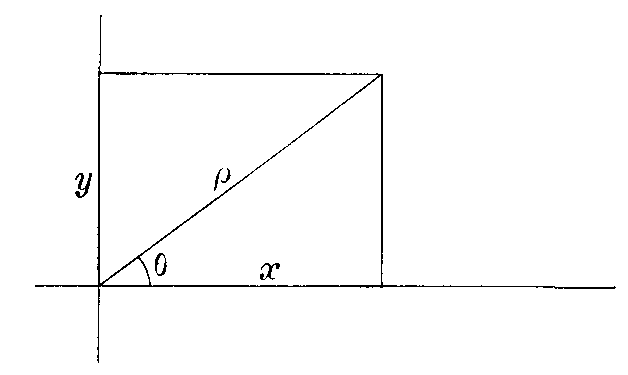
\includegraphics[width=60mm]{fig61.png}
\end{figure}

\begin{description}
\item[1.~The relations between polar and rectangular coördinates:]
\[\null\] %%ugly hack

The angles at the origin which the radius vector makes with the axes
are complementary. From the two right triangles we have

\begin{align*}
\tan ix &= \cos\theta \tan i\rho, \\
\tan iy &= \sin\theta \tan i\rho. \\
\intertext{Therefore,}
\tan^2 i\rho &= \tan^2 ix + \tan^2 iy, \\
\tan\theta &= \frac{\tan iy}{\tan ix}.
\end{align*}

\begin{figure}[h]
\centering
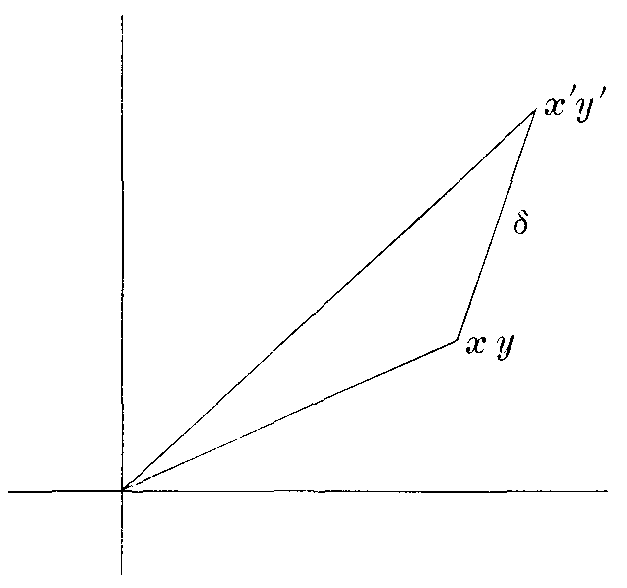
\includegraphics[width=60mm]{fig62.png}
\end{figure}

\item[2. The distance, \boldmath$\delta$, between two points:]

\begin{equation*}
\cos i\delta = \cos i\rho\, \cos i\rho'
                + \sin i\rho\, \sin i\rho'\, \cos(\theta'-\theta).
\end{equation*}
$\delta$ and one of the points being fixed, this may be regarded as
the polar equation of a circle.

\newpage
\begin{figure}[h]
\centering
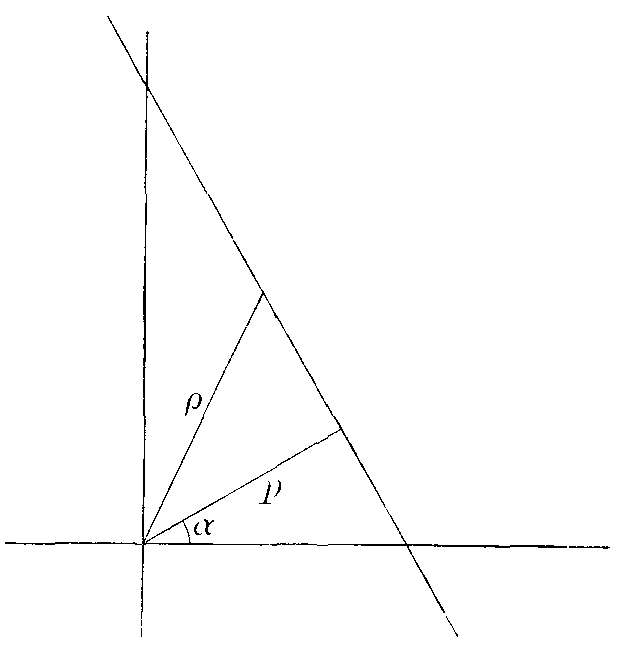
\includegraphics[width=60mm]{fig63.png}
\end{figure}

\item[3. The equation of a line:]\[\null\] %%ugly hack

\textbf{Let} $p$ be the length of the perpendicular from the origin
upon the line, and $\alpha$ the angle which the perpendicular makes
with the axis of $x$. From the right triangle formed with this
perpendicular and $\rho$ we have
\begin{equation*}
\tan i\rho\, \cos(\theta-\alpha) = \tan ip.
\end{equation*}
This is the polar equation of the line. We get the equation in $x$
and $y$ by expanding and substituting; namely,
\begin{equation*}
\cos\alpha\,\tan ix + \sin\alpha\,\tan iy = \tan ip.
\end{equation*}

\P~The equation $a\tan ix + b\tan iy = i$ represents a line for
which
\begin{equation*}
a^2 + b^2 = \frac{-1}{\tan^2 ip}.
\end{equation*}
Now, for real values of $p$, $-\tan^2ip < 1$ (see footnote,
p.~\pageref{p59ref}). The line is therefore real if $a$ and $b$ are
real, and if
\begin{equation*}
a^2 + b^2 > 1.
\end{equation*}

\newpage
\begin{figure}[h]
\centering
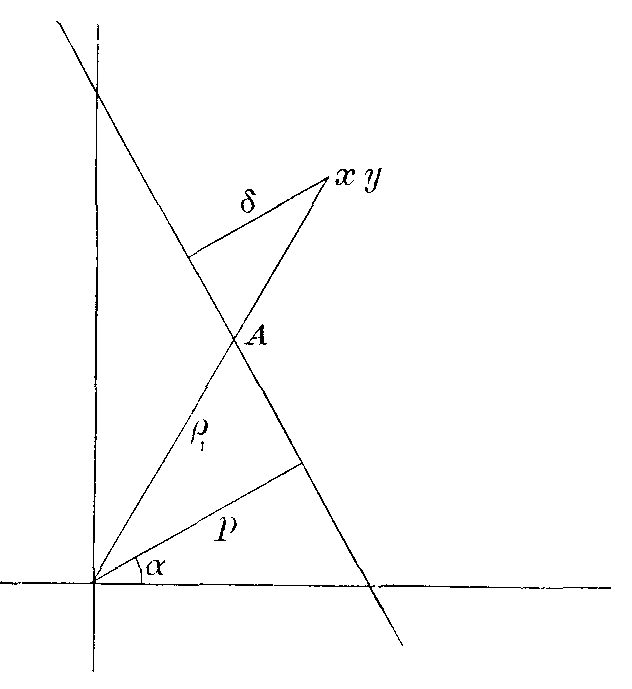
\includegraphics[width=60mm]{fig64.png}
\end{figure}

\item[4. The distance, \boldmath$\delta$, of a point from a line:]
\[\null\] %%ugly hack

\textbf{Let} the radius vector to the point intersect the line at
$A$, and let $\rho_1$ be the radius vector to $A$. We have two right
triangles with equal angles at $A$, and from the expressions for the
sines of these angles we get the equation
\begin{equation*}
\frac{\sin i\delta}{\sin i(\rho-\rho_1)} =
                                        \frac{\sin ip}{\sin i\rho_1}.
\end{equation*}
This equation holds for all points, $x\,y$, of the plane, $\delta$
being negative when the point is on the same side of the line as the
origin, and zero when the point is on the line.
\begin{equation*}
\sin i\delta
   =\frac{\sin ip}{\tan i\rho_1}\sin i\rho-\sin ip\,\cos i\rho.
\end{equation*}

Now,
\begin{align*}
\tan i\rho_1 &= \frac{\tan ip}{\cos(\theta-\alpha)}. \\
\therefore \frac{\sin ip}{\tan i\rho_1}\sin i\rho
           &=\sin i\rho\,\cos ip\,\cos(\theta-\alpha), \\
\intertext{and}
 \sin i\delta &= \cos i\rho\, \cos ip\,
   \left[\tan i\rho\, \cos(\theta-\alpha) - \tan ip\right].
\end{align*}
$\delta$ being fixed, this may be regarded as the polar equation of
an equidistant-curve.

\begin{figure}[ht]
\centering
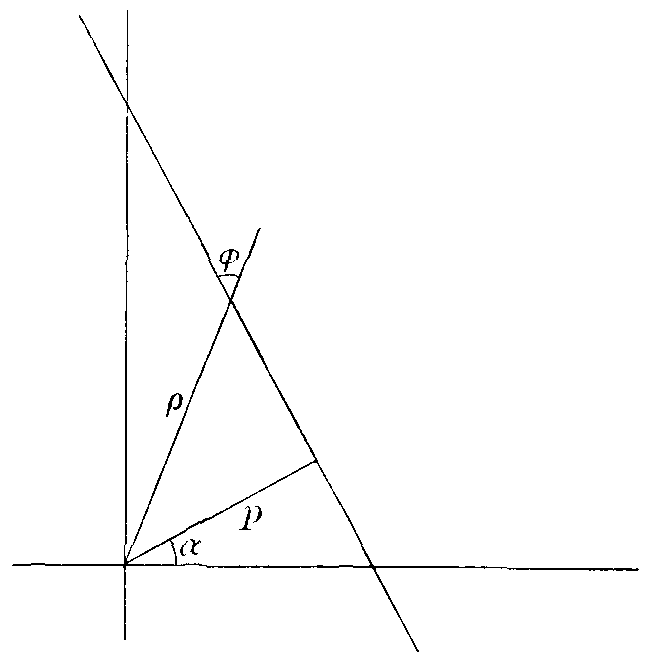
\includegraphics[width=60mm]{fig65.png}
\end{figure}

\item[5. The angle between two lines:]\[\null\] %%ugly hack

$\phi$ being the angle which a line makes with the radius vector at
any point, we have
\begin{align*}
 \cos \phi &= \cos ip\, \sin (\theta-\alpha),\\
 \sin \phi &= \frac{\sin ip}{\sin i\rho}.
\end{align*}

For two lines intersecting at this point,
\begin{align*}
 \sin \phi_1\, \sin \phi_2 &= \frac{\sin ip_1\, \sin ip_2}{\sin^2 i\rho}\\
 &= \sin ip_1\, \sin ip_2 + \frac{\sin ip_1\, \sin ip_2}{\tan^2 i\rho}.
\end{align*}

Now, from the equation of the line
\begin{align*}
\frac{\sin ip_1}{\tan i\rho} &= \cos ip_1\, \cos(\theta-\alpha_1),\\
\frac{\sin ip_2}{\tan i\rho} &= \cos ip_2\, \cos(\theta-\alpha_2);\\
\intertext{so that}
\sin \phi_1 \sin \phi_2 &= \sin ip_1\, \sin ip_2
   + \cos ip_1\, \cos ip_2\, \cos(\theta-\alpha_1)\,\cos(\theta-\alpha_2).\\
\intertext{Again,}
\cos \phi_1\, \cos \phi_2 &= \cos ip_1\, \cos ip_2\, \sin
  (\theta-\alpha_1)\,\sin (\theta-\alpha_2). \\
\intertext{Adding these equations, we have}
\cos (\phi_2-\phi_1) &= \sin ip_1\, \sin ip_2 +
        \cos ip_1\, \cos ip_2\, \cos (\alpha_2-\alpha_1).
\end{align*}

\P~Two lines are perpendicular if
\begin{align*}
\cos (\alpha_2-\alpha_1) + \tan ip_1\, \tan ip_2 &= 0. \\
\intertext{The lines}
 a \tan ix + b \tan iy &= i,\\
 a' \tan ix + b' \tan iy &= i, \\
\intertext{are perpendicular if}
aa' + bb' &=1.
\end{align*}

\item[6. The equation of a circle in $x$ and $y$:]

\begin{align*}
 \sin i\rho\, \cos \theta &= \cos i\rho\, \tan ix,\\
 \sin i\rho\, \cos \theta &= \cos i\rho\, \tan iy;
\intertext{also,}
 \cos i\rho &= \frac{1}{\sqrt{1+\tan^2 i\rho}} =
\frac{1}{\sqrt{1+\tan^2 ix+\tan^2 iy}}.
\end{align*}

The equation of a circle may, therefore, be written
\begin{multline*}
  (1 + \tan^2ix + \tan^2iy)
  (1 + \tan^2ix' + \tan^2iy') \cos^2i\delta\\
  = (1 + \tan ix \tan ix' + \tan iy \tan iy')^2.
\end{multline*}

\newpage
\begin{figure}[h]
\centering
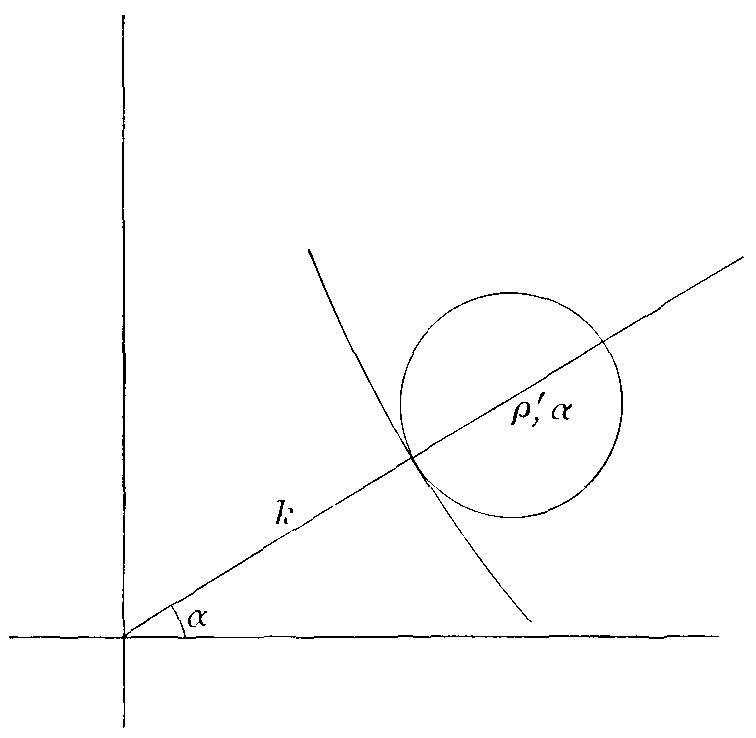
\includegraphics[width=60mm]{fig66.png}
\end{figure}

\item[7. The equation of a boundary-curve:]\[\null\] %%ugly hack

\textbf{Let} the axis of the boundary-curve which passes through the
origin make an angle, $\alpha$, with the axis of $x$, and let the
point where the boundary-curve cuts this axis be at a distance, $k$,
from the origin, positive if the origin is on the convex side of the
curve, negative if the origin is on the concave side of the curve.
The boundary-curve is the limiting position of a circle whose
centre, on this axis, moves off indefinitely.

$\rho'$ being the radius vector to the centre, the radius of the
circle is $\rho'-k$, and its equation may be written
\begin{equation*}
  \cos i(\rho'-k) = \cos i\rho\, \cos i\rho'
  + \sin i\rho\, \sin i\rho'\, \cos(\theta-\alpha),
\end{equation*}
or, expanding and dividing by $\cos i\rho'$,
\begin{equation*}
  \cos ik + \tan i\rho'\, \sin ik
  = \cos i\rho + \sin i\rho\, \tan i\rho'\, \cos(\theta-\alpha).
\end{equation*}

\P~Now, let $\rho'$ increase indefinitely. $\tan i\rho'$ tends to
the limit $i$, so that the limit of the first member of the equation
is
\begin{equation*}
  \cos ik + i\sin ik, \text{ or } e^{-k},
\end{equation*}
and the polar equation of the curve is
\begin{equation*}
  e^{-k} = \cos i\rho \left[1 + i\tan i\rho\,\cos(\theta-\alpha) \right];
\end{equation*}
or, in $x\,y$ coördinates,
\begin{equation*}
  (1 + \tan^2ix + \tan^2iy) e^{-2k}
     = (1 + i\cos\alpha\,\tan ix + i\sin\alpha\,\tan iy)^2.
\end{equation*}

\newpage
\begin{figure}[h]
\centering
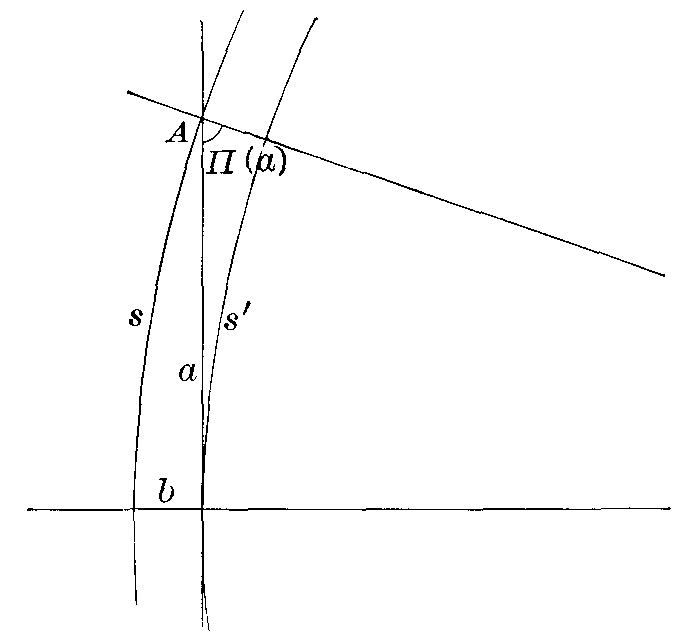
\includegraphics[width=60mm]{fig67.png}
\end{figure}

\textbf{Let} $k$ be negative and equal, say, to $-b$, and let
$\alpha=0$; also, let $a$ be the ordinate of the point $A$ where the
curve cuts the axis of $y$.

Substituting in the equation, we find
\begin{equation*}
  e^b = \cos ia.
\end{equation*}

Through $A$ draw a line parallel to the axis of $x$, and, therefore,
making an angle, $\Pi(a)$, with the axis of $y$. If we draw a
boundary-curve through the origin having the same set of parallel
lines for axes, so that the two boundary-curves cut off a distance,
$b$, on these axes, we know that the ratio of corresponding arcs is
\begin{gather*}
  \frac{s'}{s} = \sin\Pi(a) = \frac{1}{\cos ia};
\tag{See p.~\pageref{p56ref}.} \\
\intertext{therefore,}
  \frac{s'}{s} = e^{-b}.\tag{See p.~\pageref{p45ref}.}
\end{gather*}

\item[8.~The equation of an equidistant-curve:]\label{p76ref}
\[\null\] %%ugly hack

The polar equation of~(4) reduced to an equation in $x$ and $y$
takes the form
\begin{multline*}
  (1 + \tan^2ix + \tan^2iy) \sin^2i\delta \\
  = \cos^2ip (\cos\alpha\,\tan ix + \sin\alpha\, \tan iy -\tan ip)^2.
\end{multline*}

\newpage
\item[9.~Comparison of the three equations:]\[\null\] %%ugly hack

The equation
\begin{equation*}
  (1 + \tan^2ix + \tan^2iy)c^2
     = -(i-a\tan ix -b\tan iy)^2
\end{equation*}
represents a circle, a boundary-curve, or an equidistant-curve,
according as $a^2+b^2 < 1$, $=1$, $>1$, respectively.

\begin{figure}[h]
\centering
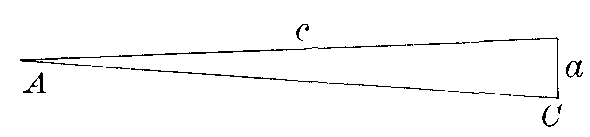
\includegraphics[width=60mm]{fig68.png}
\end{figure}

\item[10.~Differential formulæ:]\[\null\] %%ugly hack

Suppose we have an isosceles triangle in which the angle $A$ at the
vertex diminishes indefinitely. In the formula
\begin{equation*}
  \frac{\sin A}{\sin ia} = \frac{\sin C}{\sin ic}
\end{equation*}
we may put for
\begin{center}
\begin{tabular}{ccc}
  $\sin A$, & $\sin ia$, & $\sin C$;\\
  $A$, & $ia$, & $1$,\\
\end{tabular}\\
\end{center}
respectively. Therefore,
\begin{equation*}
  ia = \sin ic \cdot A.\tag{I.}
\end{equation*}

\textbf{Corollary.} \emph{In a circle of radius $\mathbf{r}$, the
ratio of any arc to the angle subtended at the centre is $\sin
\mathbf{ir}$.}

\begin{figure}[h]
\centering
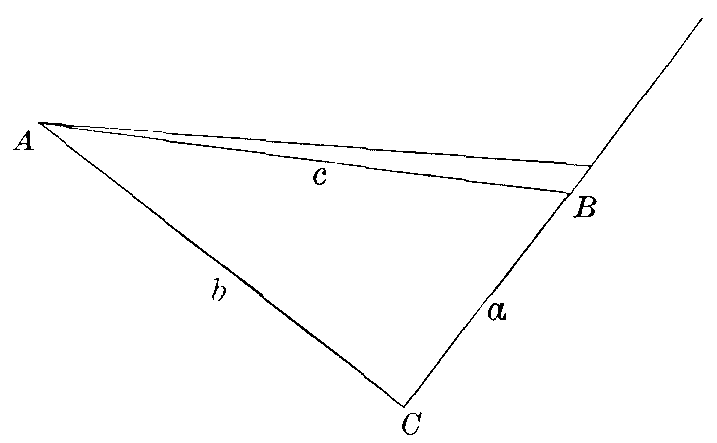
\includegraphics[width=60mm]{fig69.png}
\end{figure}

Again, in the right triangle $ABC$, let the hypothenuse $c$ revolve
about the vertex $A$. Differentiating the equation
\begin{align*}
\sin A &= \frac{\cos B}{\cos ib},  \\
\intertext{where $b$ is constant, we have }
\cos Ad\,A &= -\,\frac{\sin B\,dB}{\cos ib}.  \\
\intertext{But }
\sin B &= \frac{\cos A}{\cos ia};  \\
\therefore dB &= -\cos ia\, \cos ib\, dA,  \\
\intertext{or (II.) }
dB &= -\cos ic\, dA.
\end{align*}

\P~Now, using polar coördinates, we have an infinitesimal right
triangle whose hypothenuse, $ds$, makes an angle, say $\phi$, with
the radius vector (see figure on page~\pageref{p78fig}). The two
sides about the right angle are $d\rho$ and $\frac{\sin i\rho}{i}
d\theta$; therefore,
\begin{align*}
ds^2 &= d\rho^2 - \sin^2i\rho\, d\theta^2,  \\
\tan\phi &= \frac{\sin i\rho}{i}\, \frac{d\theta}{d\rho}.
\end{align*}

\begin{figure}[h]
\centering
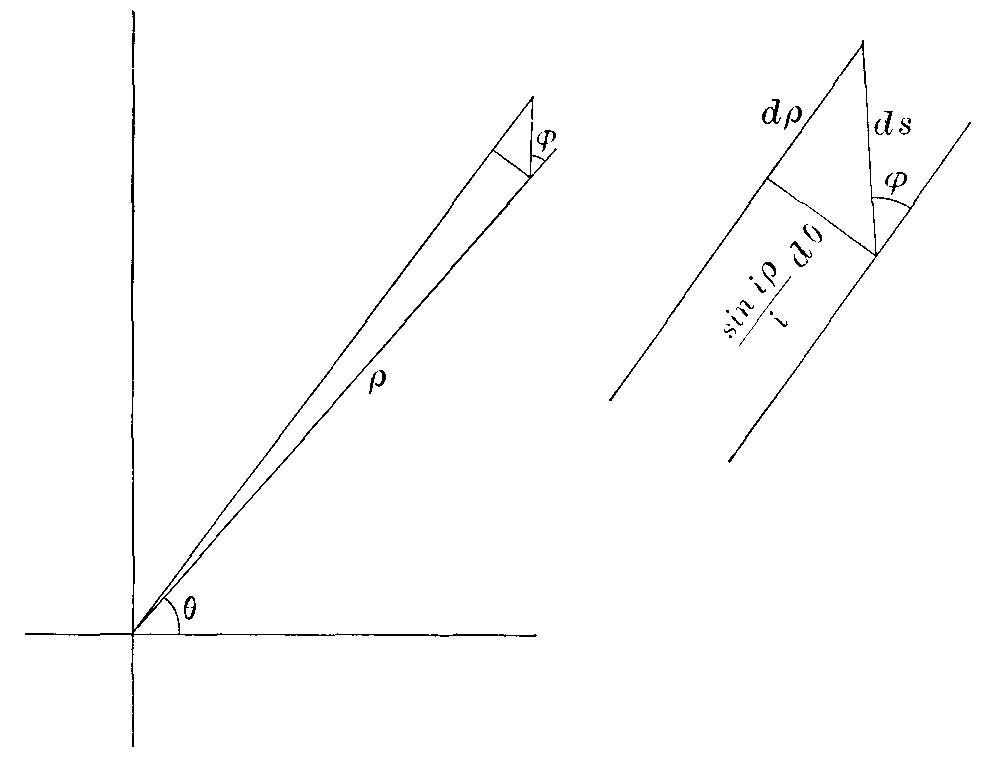
\includegraphics[width=80mm]{fig70.png}
\end{figure}

\label{p78fig}For two arcs cutting at right angles, let $d'$ denote
differentiation along the second arc:
\begin{align*}
  \frac{\sin i\rho}{i}\, \frac{d\theta}{\rho}
  &= -\, \frac{i}{\sin i\rho}\, \frac{d'\rho}{d'\theta},\\
\intertext{or}
  \frac{d\rho}{d\theta}\, \frac{d'\rho}{d'\theta}
  &= \sin^2i\rho.
\end{align*}

\item[11.~Area:]\[\null\] %%ugly hack

It equals
\begin{equation*}
  \iint \frac{\sin i\rho}{i}\, d\rho\, d\theta.\footnotemark
\end{equation*}
\footnotetext{The unit of area being so chosen that the area of an
infinitesimal rectangle may be expressed as the product of its base
and altitude.}

We will consider only the case where the origin is within the area
to be computed and where each radius vector meets the bounding curve
once, and only once.

Integrating with respect to $\rho$, from $\rho=0$, we have
\begin{align*}
  \int_0^{2\pi} (\cos i\rho - 1) d\theta,\\
  \intertext{or}
  \int_0^{2\pi} \cos i\rho\, d\theta - 2\pi.
\end{align*}

\begin{figure}[h]
\centering
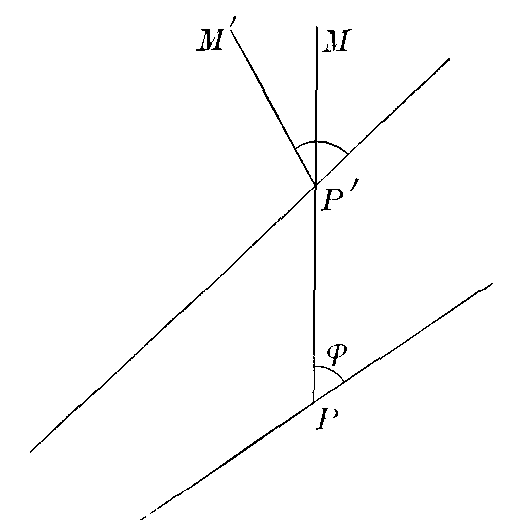
\includegraphics[width=60mm]{fig71.png}
\end{figure}

Suppose $P$ and $P'$ are two ``consecutive'' points on the curve,
$PM$ and $P'M'$ the tangents at these points, and $\phi$ the angle
which the tangent makes with the radius vector. The angle $MP'M'$
indicates the amount of turning or rotation at these points as we go
around the curve.

\P~Now, by~(II.),
\begin{equation*}
  MP'M' = d\phi + \cos i\rho\, d\theta.
\end{equation*}

\label{p79ref}\P~In going around the curve, $\phi$ may vary but
finally returns to its original value. That is, for our curve
\begin{gather*}
  \int d\phi = 0, \\
\intertext{and the amount of rotation is}
  \int_0^{2\pi} \cos i\rho\, d\theta.
\end{gather*}

Hence, the area is equal to the excess over four right angles in the
amount of rotation as we go around the curve. This theorem can be
extended to any finite area.

\item[12. A modified system of coördinates:]\[\null\] %%ugly hack

Our equations take simple forms if we write $iu$ for $\tan ix$, $iv$
for $\tan iy$, $ir$ for $\tan i\rho$, and so on for all lengths of
lines.

Thus, we have
\begin{align*}
u^2 + v^2 &= r^2.\footnotemark \\
\intertext{The equation of a line is}
au + bv &= 1, \\
\intertext{and the equation}
(1 - u^2 - v^2)c^2 &= (1 - au - bv)^2
\end{align*}
represents a circle, a boundary-curve, or an equidistant-curve,
according as $a^2+b^2<1$, $=1$, $>1$, respectively.
\footnotetext{If we draw a quadrilateral with three right angles and
the diagonal to the acute angle, and use $a$, $b$, and $c$ in the
same way that $u$, $v$, and $r$ are used above, the five parts
lettered in the figure have the relations of a right triangle in the
Euclidean Geometry; \emph{e.g.},
\begin{equation*}
a^2 + b^2 = c^2 , \sin A = \frac{a}{c}, \text{etc}.
\end{equation*}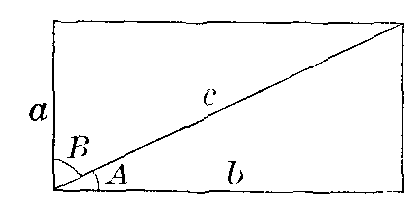
\includegraphics[width=25mm]{fig73.png}}\label{p80fn}
\end{description}

\section{Elliptic Analytic Geometry}

The Elliptic Analytic Geometry may be developed just as we have
developed the Hyperbolic Analytic Geometry, and the formulæ are the
same with the omission of the factor $i$. But these formulæ are also
very easily obtained from the relation of line and pole, and we
shall produce them in this way.

The formulæ of Elliptic Plane Analytic Geometry may be applied to a
sphere in any of our three Geometries.

\begin{figure}[h]
\centering
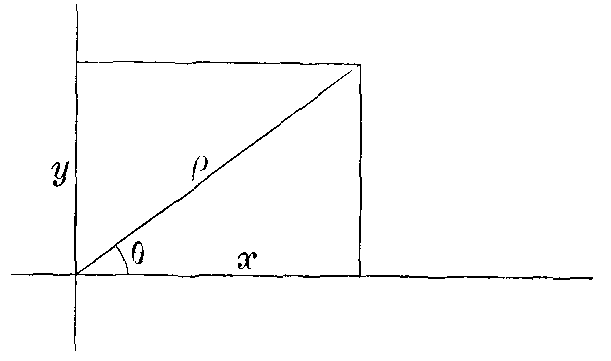
\includegraphics[width=60mm]{fig72.png}
\end{figure}

\begin{description}
\item[1. The relations between polar and rectangular coördinates:]

\begin{gather*}
\tan x = \cos\theta\, \tan\rho, \quad \tan y = \sin\theta\, \tan\rho; \\
\intertext{therefore,}
\begin{aligned}
  \tan^2\rho &= \tan^2x + \tan^2y,\\
  \tan\theta &= \frac{\tan y}{\tan x}.\footnotemark
\end{aligned}
\end{gather*}
\footnotetext{The line which has the origin for pole forms with the
coördinate axes a trirectangular triangle, and $x$, $y$, and
$\theta$ may be regarded as representing the directions of the given
point from its three vertices.
\par On a sphere, if we take as origin the pole of the equator, $\rho$
and $\theta$ are colatitude and longitude. $x$ and $y$, one with its
sign changed, are the ``bearings'' of the point from two points
$90^\circ$ apart on the equator.}

\newpage
\begin{figure}[h]
\centering
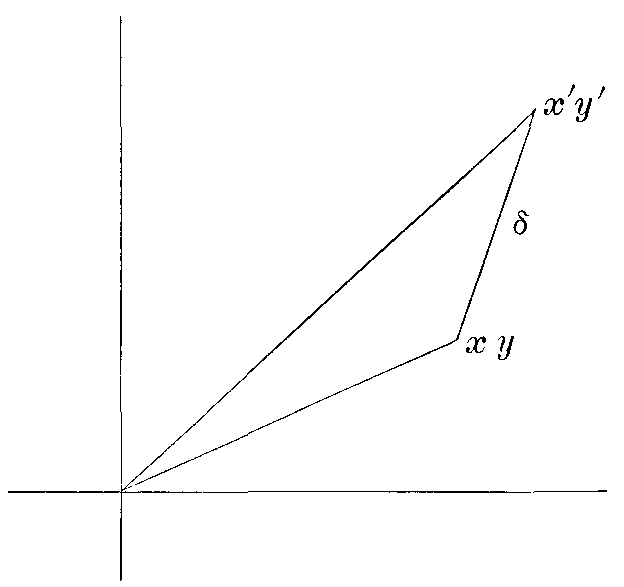
\includegraphics[width=60mm]{fig74.png}
\end{figure}

\item[2. The distance, \boldmath$\delta$, between two points:]

\begin{equation*}
\cos\delta = \cos\rho\,\cos\rho' +
                             \sin\rho\,\sin\rho'\cos(\theta'-\theta).
\end{equation*}

This may be regarded as the polar equation of a circle of radius
$\delta$, $\rho'$ and $\theta'$ being the polar coördinates of the
centre.

Now,
\begin{align*}
  \sin\rho\,\cos\theta &= \cos\rho\,\tan x,\\
  \sin\rho\,\sin\theta &= \cos\rho\,\tan y;
\intertext{also,}
  \cos\rho = \frac{1}{\sqrt{1+\tan^2\rho}}
  &= \frac{1}{\sqrt{1+\tan^2x+\tan^2y}}
\end{align*}
The equation of a circle in rectangular coördinates may, therefore,
be written
\begin{multline*}
  (1 + \tan^2x + \tan^2y) (1 + \tan^2x' + \tan^2y') \cos^2\delta\\
  = (1 + \tan x\tan x' + \tan y\tan y')^2.
\end{multline*}

\newpage
\begin{figure}[h]
\centering
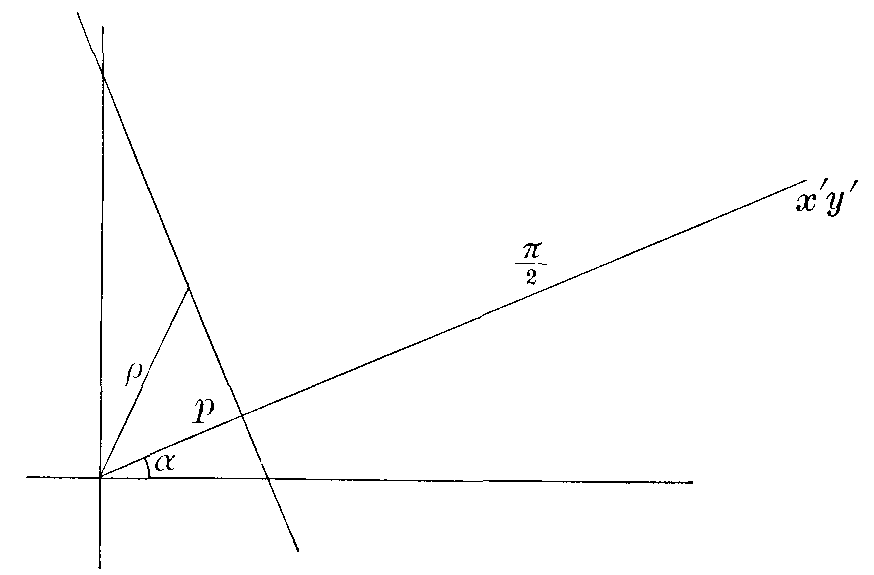
\includegraphics[width=60mm]{fig75.png}
\end{figure}

\item[3. The equation of a line:]\[\null\] %%ugly hack

When $\delta = \nicefrac{\pi}{2}$, the circle becomes a straight
line. For this we have, therefore, the equation
\begin{equation*}
  \tan x \tan x' + \tan y \tan y' + 1 = 0.
\end{equation*}
$x'y'$ is the pole of the line.

From the equation
\begin{align*}
\tan\rho\, \cos(\theta-\alpha) &= \tan p, \\
\intertext{or}
\cos\alpha\, \tan x + \sin\alpha\,\tan y &= \tan p, \\
\intertext{we find}
\tan x' &= -\frac{\cos\alpha}{\tan p},\\
\tan y' &= -\frac{\sin\alpha}{\tan p},
\end{align*}
as can be shown geometrically, the polar coördinates of this point
being
\begin{equation*}
p+\frac{\pi}{2},\ \alpha.
\end{equation*}

The equation
\begin{equation*}
  a\tan x + b\tan y + 1 = 0
\end{equation*}
represents a real line for any real values of $a$ and $b$.

\newpage
\item[4. The distance, \boldmath$\delta$, of a point from a
straight line:]\[\null\] %%ugly hack

This is the complement of the distance between the point and the
pole of the line; it is expressed by the equation
\begin{align*}
  \sin\delta &= -\cos\rho\,\sin p
                            + \sin\rho\,\cos p\,\cos(\theta-\alpha)\\
  &= \cos\rho\,\cos p
                 \left[\tan\rho\,\cos(\theta-\alpha) - \tan p\right].
\end{align*}

\item[5. The angle, \boldmath$\phi$, between two lines:]
\[\null\] %%ugly hack

This is equal to the distance between their poles; therefore,
\begin{equation*}
  \cos\phi = \sin p\,\sin p' + \cos p\,\cos p'\,\cos(\alpha'-\alpha).
\end{equation*}

The two lines
\begin{align*}
  a\phantom{'}\tan x + b\phantom{'}\tan y + 1 &= 0,\\
  a'\tan x + b'\tan y + 1 &= 0\\
  \intertext{are perpendicular if}
  aa' + bb' + 1 &= 0.
\end{align*}

\begin{figure}[h]
\centering
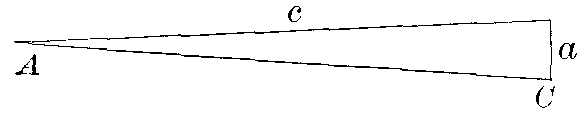
\includegraphics[width=60mm]{fig76.png}
\end{figure}

\item[6. Differential formulæ:]\[\null\] %%ugly hack

The formula
\begin{equation*}
  \frac{\sin A}{\sin a} = \frac{\sin C}{\sin c}
\end{equation*}
becomes, when $A$ diminishes indefinitely,
\begin{equation*}
  a = \sin c \cdot A.\tag{I.}
\end{equation*}

\newpage
\label{p83ref}\textbf{Corollary.} \emph{In a circle of radius
$\mathbf{r}$, the ratio of any arc, to the angle subtended at the
centre is $\sin \mathbf{r}$.}

\begin{figure}[h]
\centering
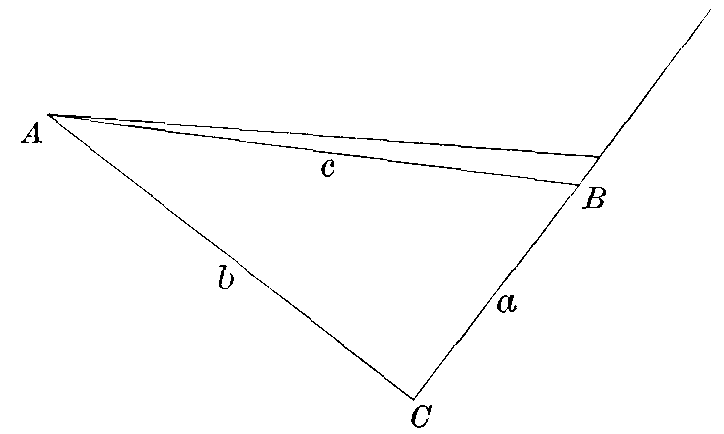
\includegraphics[width=60mm]{fig77.png}
\end{figure}

From the right triangle $ABC$, if $b$ remain fixed, we get, by
differentiating the equation
\begin{align*}
  \sin A &= \frac{\cos B}{\cos b}, \\
  dB &= -\cos c \,dA.\tag{II.}
\end{align*}

\begin{figure}[h]
\centering
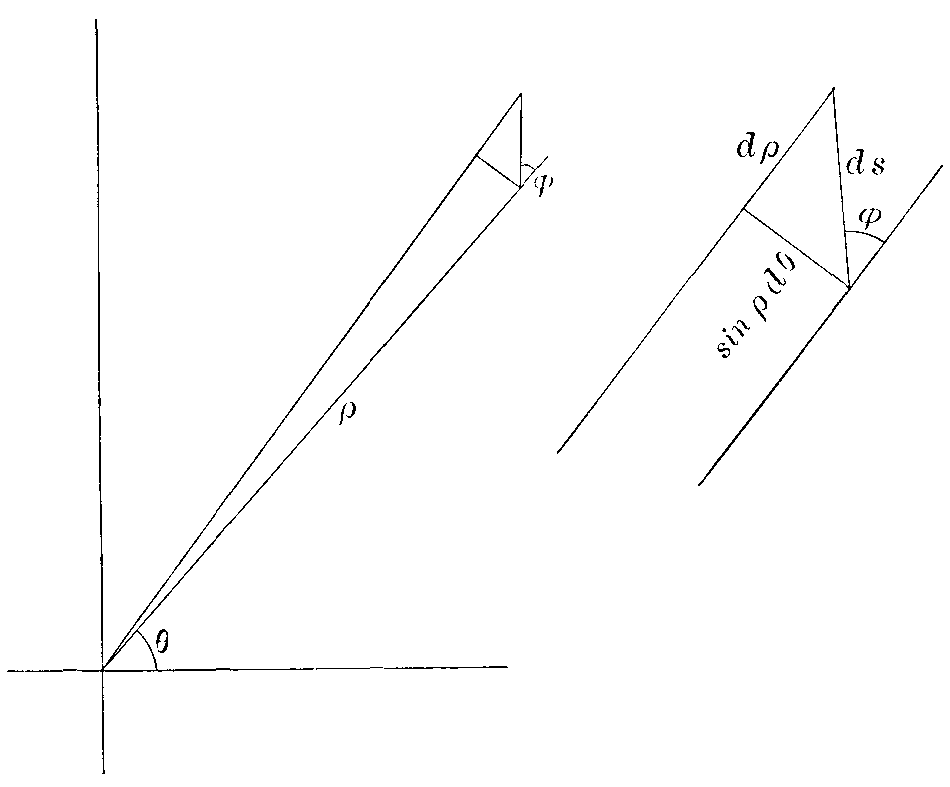
\includegraphics[width=80mm]{fig78.png}
\end{figure}

\newpage
Thus, we have for differential formulæ in polar coördinates
\begin{align*}
  ds^2 &= d\rho^2 + \sin^2\rho\,d\theta^2,\\
  \tan\phi &= \sin\rho\, \frac{d\theta}{d\rho};\footnotemark
\intertext{and for two arcs cutting at right angles}
  \frac{d\rho}{d\theta}\, \frac{d'\rho}{d'\theta} &= -\sin^2\rho.
\end{align*}
\footnotetext{If $\phi$ is constant, as in the logarithmic spiral of
Euclidean Geometry, we can integrate this equation; namely,
  \begin{align*}
    \tan\phi\, \frac{d\rho}{\sin\rho} &= d\theta.\\
    \therefore \tan\phi\, \log\tan\frac{\rho}{2} &= \theta+c,\\
    \intertext{or}
    \tan\frac{\rho}{2} &= e^\frac{\theta+c}{\tan\phi}.\\
    \intertext{Writing $c'$ for $e^\frac{c}{\tan\phi}$, this is}
    \tan\frac{\rho}{2} &= c' e^\frac{\theta}{\tan\phi}.
  \end{align*}
  On the sphere this is the curve called the loxodrome.}

The formula for area is\footnote{The unit of area being properly chosen.}
\begin{equation*}
  \iint \sin\rho\, d\rho\, d\theta.
\end{equation*}
We integrate first with respect to $\rho$, and if the area contains
the origin and each radius vector meets the curve once, and only
once, our expression becomes
\begin{equation*}
  2\pi - \int_0^{2\pi} \cos\rho\, d\theta.
\end{equation*}

The entire rotation in going around the curve is found as on
page~\pageref{p79ref}, and is
\begin{equation*}
  \int_0^{2\pi} \cos\rho\, d\theta.
\end{equation*}
Thus the area is equal to the amount by which this rotation is less
than four right angles.

For example, the area of a circle of radius $\rho$ is
$2\pi(1-\cos\rho)$, and the amount of turning in going around it is
$2\pi\cos\rho$. The area of the entire plane is $2\pi$.

\item[7. A modified system of coördinates:]\[\null\] %%ugly hack

Writing $u$ for $\tan x$, $v$ for $\tan y$, $r$ for $\tan\rho$,
etc., we have
\begin{align*}
  u^2 + v^2 &= r^2.\footnotemark \\
\intertext{The equation of a line then becomes}
  au + bv + 1 &= 0, \\
\intertext{and the equation of a circle}
  (1 + u^2 + v^2)c^2 &= (1 + au + bv)^2.
\end{align*}
\footnotetext{The footnote on page~\pageref{p80fn} applies here
also.}
\end{description}

\section{Elliptic Solid Analytic Geometry}

We will develop far enough to get the equation of the surface of
double revolution.

\begin{figure}[h]
\centering
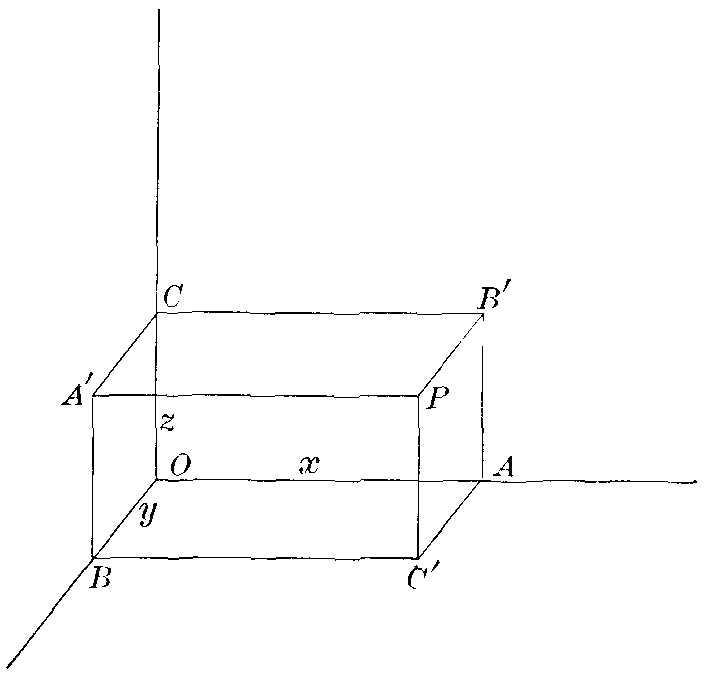
\includegraphics[width=60mm]{fig79.png}
\end{figure}

\begin{description}
\item[1. Coördinates, lines, and planes:]\[\null\] %%ugly hack

Draw three planes through the point perpendicular to the axes. For
co\-ör\-din\-ates $x$, $y$, $z$, we take the intercepts which these
planes make on the axes.

The lines of intersection of these three planes are perpendicular to
the coördinate planes (Chap.~I, II, 16 and 17); in fact, all the
face angles in the figure are right angles except those at $P$ and
the three angles $BA'C$, $CB'A$, and $AC'B$, which are obtuse
angles.

Let $\rho$ be the radius vector to the point $P$, and $\alpha$,
$\beta$, and $\gamma$ the three angles which it makes with the three
axes. Then
\begin{align*}
  \cos^2\alpha + \cos^2\beta + \cos^2\gamma &= 1,\\
  \cos\alpha &= \frac{\tan x}{\tan\rho},\ \text{etc.;}\\
  \tan^2x + \tan^2y + \tan^2z &= \tan^2\rho.
\end{align*}

For the angle between two lines intersecting at the origin
\begin{equation*}
  \cos\theta = \cos\alpha\,\cos\alpha' + \cos\beta\,\cos\beta'
  + \cos\gamma\,\cos\gamma'.
\end{equation*}

The angle subtended at the origin by the two points $xyz$ and
$x'y'z'$ is given by the equation
\begin{equation*}
  \cos\theta = \frac{\tan x\, \tan x' + \tan y\, \tan y'
    + \tan z\, \tan z'}{\tan\rho\, \tan\rho'}.
\end{equation*}

For the distance between two points
\begin{equation*}
  \cos\delta = \cos\rho\,\cos\rho' + \sin\rho\,\sin\rho'\,\cos\theta.
\end{equation*}

This gives us the equation of a sphere, and for $\delta =
\nicefrac{\pi}{2}$ the equation of a plane. The latter in
rectangular coördinates is
\begin{equation*}
  \tan x\, \tan x' + \tan y\, \tan y' + \tan z\, \tan z' + 1 = 0.
\end{equation*}

Let $p$ be the length of the perpendicular from the origin upon the
plane, and $\alpha$, $\beta$, $\gamma$ the angles which this
perpendicular makes with the axes. Then we have for its pole
\begin{align*}
  \rho' &= p + \frac{\pi}{2},\\
  \tan x' = \tan\rho'\,\cos\alpha &= -\,\frac{\cos\alpha}{\tan p},\
  \text{etc.;}
\end{align*}
hence, the equation of the plane may be written
\begin{equation*}
\cos\alpha\,\tan x + \cos\beta\,\tan y + \cos\gamma\,\tan z
   = \tan p.
\end{equation*}

\newpage
\item[2. The surface of double revolution:]\[\null\] %%ugly hack

Take one of its axes for the axis of $z$, suppose $k$ the distance
of the surface from this axis, and let $\theta$ denote the angle
which the plane through the point $P$ and the axis of $z$ makes with
the plane of $xz$. We may call $z$ and $\theta$ latitude and
longitude.

Produce $OA$ and $CB$. They will meet at a distance,
$\nicefrac{\pi}{2}$, from the axis of $z$ in a point, $O'$, on the
other axis of the surface, and there form an angle that is equal in
measure to $z$.

From the right triangle $O'AB$
\begin{align*}
\cos z &= \frac{\tan OA}{\tan O'B}.\\
\intertext{But}
\tan O'A &= \cot x,\\
\intertext{and}
\tan O'B &= \cot CB = \frac{\cot k}{\cos\theta}.\\
\intertext{Therefore,}
\cos z &= \frac{\tan k\,\cos\theta}{\tan x},\\
\intertext{or}
\tan x &= \frac{\tan k\,\cos\theta}{\cos z}.\\
\intertext{Similarly,}
\tan y &= \frac{\tan k\,\sin\theta}{\cos z}.\\
\intertext{Squaring and adding, we have for the equation of the
  surface}
\tan^2x + \tan^2y &= \tan^2k\sec^2z.
\end{align*}

\newpage
\begin{figure}[h]
\centering
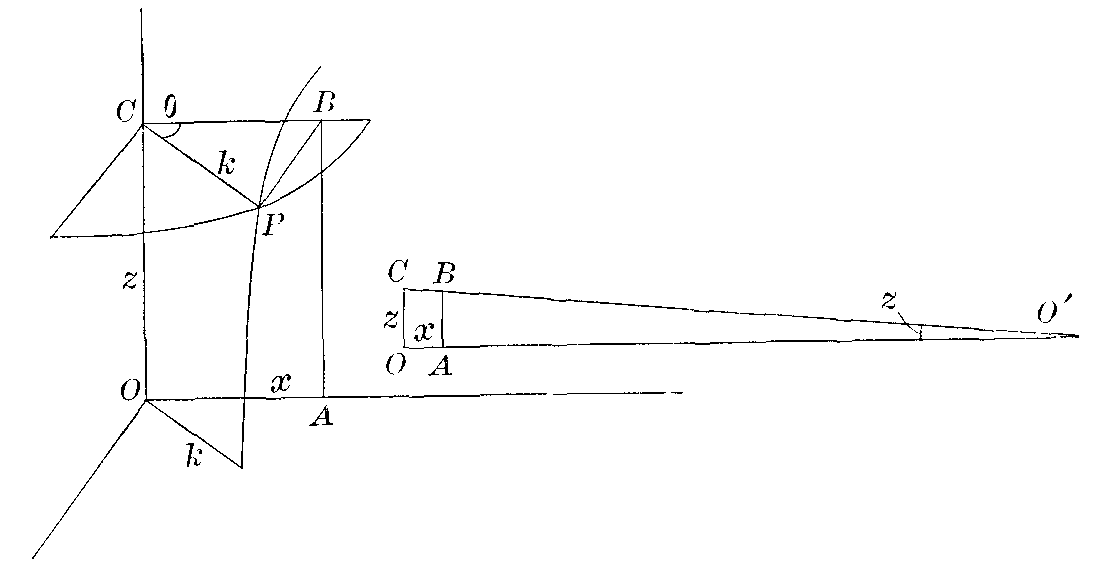
\includegraphics[width=80mm]{fig80.png}
\end{figure}

For the length of the chord joining two points on the surface, we
have
\begin{equation*}
\cos\delta = \cos\rho\,\cos\rho'
  (1 + \tan x\,\tan x' + \tan y\,\tan y' + \tan z\,\tan z').
\end{equation*}
Now,
\begin{align*}
\tan^{2}\rho &= \tan^{2}k\,\sec^{2}z + \tan^{2}z; \\
\intertext{therefore,}
\sec^{2}\rho &= \sec^{2}k\,\sec^{2}z,\\
\intertext{or}
\cos\rho &= \cos k\,\cos z. \\
\intertext{That is, in terms of $z$, $z'$, $\theta$, and $\theta'$,
we have}
\cos\delta &= \cos^2k\,\cos(z'-z) + \sin^2k\,\cos(\theta'-\theta). \\
\intertext{From this we can get an expression for $ds$, the
differential element of length on the surface:}
\cos ds &= \cos^2k\,\cos dz + \sin^2k\,\cos d\theta, \\
\intertext{or, since}
\cos ds &= 1 - \frac{ds^2}{2},\ \text{etc.,} \\
ds^2 &= \cos^2k\, dz^2 + \sin^2k\, d\theta^2.
\end{align*}

$z$ and $\theta$ are proportional to the distances measured along
the two systems of circles. These circles cut at right angles, and
may be used to give us a system of rectangular coördinates on the
surface. The actual lengths along these two systems of circles are
$\theta\sin k$ and $z\cos k$ (see Cor.~p.~\pageref{p83ref}). If,
therefore, we write
\begin{equation*}
\alpha = \theta\sin k,\quad \beta = z\cos k,
\end{equation*}
we shall have a rectangular system on the surface where the
coördinates are the distances measured along these two systems of
circles which cut at right angles.

The formula now becomes
\begin{equation*}
ds^2 = d\alpha^2 + d\beta^2.
\end{equation*}

An equation of the first degree in $\alpha$ and $\beta$ represents a
curve which enjoys on this surface all the properties of the
straight line in the plane of the Euclidean Geometry. Through any
two points one, and only one, such line can be drawn, because two
sets of coördinates are just sufficient to determine the
coefficients of an equation of the first degree. The shortest
distance between two points on the surface is measured on such a
line. For, the distance between two points on a path represented by
an equation in $\alpha$ and $\beta$ is the same as the distance
between the corresponding points and on the corresponding path in a
Euclidean plane in which we take $\alpha$ and $\beta$ for
rectangular coördinates. It must, therefore, be the shortest when
the path is represented by an equation of the first degree in
$\alpha$ and $\beta$. Such a line on a surface is called a
\emph{geodesic line}, or, so far as the surface is concerned, a
straight line. The distance between any two points measured on one
of these lines is expressed by the formula
\begin{equation*}
d = \sqrt{(\alpha-\alpha')^2 + (\beta-\beta')^2}.
\end{equation*}

Triangles formed of these lines have all the properties of plane
triangles in the Euclidean Geometry: the sum of the angles is $\pi$,
etc. In fact this surface has the same relation to elliptic space
that the boundary-surface has to hyperbolic space.

The normal form of the equation of a line is
\begin{equation*}
\alpha\cos\omega + \beta\sin\omega = p.
\end{equation*}

The rectilinear generators of the surface make a constant angle,
$\pm k$, with all the circles drawn around the axis which is polar
to the axis of $z$. These generators are then ``straight lines'' on
the surface, and their equation takes the form
\begin{equation*}
\alpha\cos k \pm \beta\sin k = p.
\end{equation*}
\end{description}

